% udf.tex
\section{User-defined functions for run-time customization}
\label{udf-sec}
User-defined functions (UDFs) are callable functions written in Lua
that are used to perform specialized and/or customized tasks.\footnote{Note that the following information 
is likely to become dated with code changes,
so it is best to refer to the actual source code to see what is expected.
Look in \texttt{bc\_user\_defined.cxx} for the boundary condition functions and \texttt{main.cxx} for the 
functions related to source terms.}
These callable functions can be used for:
\begin{itemize}
\item specialized boundary conditions;
\item the addition of custom source terms; and
\item to perform special operations at the beginning and end of each timestep.
\end{itemize}
Some examples follow to give this idea a more concrete form.
A specialized boundary condition might model mass injection
from a porous boundary which is not presently available as a boundary condition
in the simulation code.
We use custom source terms when we are testing the code using the
method of manufactured solutions (see Sections~\ref{mms-euler-sec} and \ref{mms-viscous-sec}).
The callable functions at the start and end of each timestep could be used
to compute a special flow field variable.

\subsection{Customizing the boundary conditions}
\index{boundary conditions!user defined}
Using a customized boundary condition requires two steps:
\begin{enumerate}
\item Selecting the \texttt{UserDefinedBC()} in the block setup.
\item Constructing a Lua file which defines the boundary condition behaviour.
\end{enumerate}

When the user's (Python) input script calls up a \texttt{UserDefinedBC()} boundary condition,
a Lua file is specified.
This file is run at the time of boundary-condition instantiation and it needs to define the
Lua functions \texttt{ghost\_cell(args)} and \texttt{interface(args)} at a minimum.
These functions are later called, every time the boundary condition is applied during the simulation.
As well as providing the \textit{expected} functions, the Lua file may contain whatever else
the user wishes.
It may start up external processes, read data files, or any other suitable activity that
sets up data for later use in the boundary condition functions.

When using the user-defined boundary conditions you need to instruct the code about 
what to do for the convective (inviscid) update and then, separately, for the viscous effects. 
The inviscid interaction at the boundary may be handled in one of two ways:
\begin{enumerate}
 \item Defining a \verb!ghost_cell()! function.\\
  In this case, you populate the properties of two ghost cells such that 
  they give the desired inviscid effect at the wall. 
  The ghost cells are abstract in that they do not exist in the simulated flow domain
  but do exist in the code data for each block boundary. 
  They are used in the interpolation phase of the convective update,
  for cell faces that lie along the boundary.
  For the case of a solid wall, you use the \verb!ghost_cell()! function 
  and reflect the normal velocity.
  Examples of this are in the test cases.
 \item Defining a \verb!convective_flux()! function. \\
  This is an alternative to the \verb!ghost_cell()! function and
  allows you to directly specify the convective flux. 
  This function is only used if the \verb!sets_conv_flux_flag! is set in the boundary condition. 
  If it is set, the \verb!convective_flux()! function will override anything in the \verb!ghost_cell()! function
  thus causing the \verb!ghost_cell()! function to have no effect (however, it is still needs to be present due to the
  way the implementation works).
\end{enumerate}

The viscous effects at the boundary are also handled in one of two ways:
\begin{enumerate}
 \item Defining an \verb!interface()! function.\\
  In this case, you set the properties at the interface directly
  and, as part of the viscous update, the main code computes spatial derivatives from these specified
  flow properties. 
  For example, you could set a temperature at the interface and zero velocity for a no-slip wall
  with the function called \verb!interface()!. 
  By doing this, you would not directly control the viscous heat flux into the flow directly, 
  however, it would be controlled indirectly by setting the temperature.
 \item Defining a \verb!viscous_flux()! function. \\
  The other option is to specify the viscous flux directly at the boundary.
  The function inputs and outputs are identical to the \verb!convective_flux()! function,
  except that the values for viscous fluxes of conserved quantities are returned.
  This option is convenient when something is directly known about the viscous
  flux effect at the boundary.
  For example, a heat flux at the boundary may be specified directly using this
  user-defined function.
  This function is only used if the \verb!sets_visc_flux_flag! is set in the boundary condition,
  otherwise the code will just look to apply the \verb!interface()! function.
\end{enumerate}
Note that in an inviscid simulation, any user-specied viscous boundary effect functions
are ignored: they are never called by the code.

\medskip
The Lua execution environment provided to the file includes the following data:\\
\vspace{1mm}
\begin{tabular}{ll} 
 \hline \noalign{\smallskip}
 \texttt{block\_id} & \parbox{10cm}{index of the current block. 
                                   Boundary conditions exist in the context a block.
                                   This means that the information accessible from the UDFs is limited
                                   to that contained within the block plus a little bit of global data.
                                   This is particularly important for parallel (MPI) simulations
                                   because blocks exist is separate processes and the data in one
                                   block is not generally available in another.} \\ \hline
 \texttt{nsp} & number of species \\
 \texttt{nmodes} & number of energy storage modes (and temperatures) \\
 \texttt{nni,nnj,nnk} &  number of cells in each index direction for the current block \\
 \noalign{\smallskip} \hline \noalign{\smallskip}
 \texttt{NORTH} & \parbox{10cm}{index of the ``North'' boundary.
                               This index (and the following indices) will be handy for deciding which boundary we are
                               working on when the \texttt{ghost\_cell(args)} and \texttt{interface(args)} 
                               are called.}\\
 \texttt{EAST,SOUTH,WEST} &  \\
 \texttt{TOP,BOTTOM} &  \\
 \noalign{\smallskip} \hline \noalign{\smallskip}
\end{tabular}

\noindent
As well as the data, there are a couple of functions that can be called to get more information about
the flow at specific locations:\\
\begin{tabular}{ll} 
 \noalign{\smallskip} \hline \noalign{\smallskip}
 \texttt{sample\_flow(jb,i,j,k)} & \parbox{10cm}{a function that returns a table of 
                                      the flow state for a particular cell.  The data is the same as that
                                      listed for the \texttt{ghost\_cell} tables (see below) with the addition of \texttt{vol},
                                      the cell volume.  This function is not likely to work for a MPI simulation,
                                      where only one block is visible to the current process.

                                      This function may be called with indices which sample the properties
                                      in the ghost cells themselves. When this is the case, the flow properties
                                      in the ghost cells should not be relied on. The only useful data is
                                      the position (\texttt{x}, \texttt{y} and \texttt{z}) and the volume
                                      \texttt{vol}. These values are estimated by using a linear extrapolation
                                      from the nearby interior cells. The values of position and volume may
                                      be useful when setting the properties in the ghost cells (see for
                                      example the application in MMS case to give a first-order boundary
                                      condition).
                                                                             

} \\
 \texttt{sample\_i\_face(jb,i,j,k)} & \parbox{10cm}{a function that returns a table of 
                                      the flow state for a particular I-interface.  The data is the same as that
                                      listed for the \texttt{ghost\_cell} tables with the addition of \texttt{length},
                                      the interface.  This function is not likely to work for a MPI simulation,
                                      where only one block is visible to the current process.
} \\
 \texttt{sample\_j\_face(jb,i,j,k)} & \parbox{10cm}{As for \texttt{sample\_i\_face()} except that the properties
                                      are returned for a J-interface.
} \\
 \texttt{sample\_k\_face(jb,i,j,k)} & \parbox{10cm}{As for \texttt{sample\_i\_face()} except that the properties
                                      are returned for a K-interface.
} \\
 \noalign{\smallskip} \hline \noalign{\smallskip}
 \texttt{locate\_cell(x,y,z)} & \parbox{10cm}{a function that will search for the cell nearest 
                                      the specified coordinates and return the cell indices
                                      and the index of the containing block.  This function 
                                      is not likely to work for a MPI simulation,
                                      where only one block is visible to the current process.} \\
 \noalign{\smallskip} \hline \noalign{\smallskip}
\end{tabular}

\noindent

There are some additional convenience functions available to the user to compute or obtain
values related to the gas model such as thermodynamic properties and transport coefficients.
These are discussed in detail in Section~\ref{sec:udf-gas-service}.

\medskip
On being called at run time, the function \texttt{ghost\_cell(args)} returns two Lua tables.
It is the user writing the function who is responsible for constructing and returning
these two tables.
The first contains the flow state in the ghost cell nearest the boundary face, 
and the second contains the flow state for the ghost cell further away from the boundary face.
Items to appear in the returned tables are:\\
\begin{tabular}{lp{12cm}}
 \texttt{p} &  gas pressure \\
 \texttt{u,v,w} & velocity components in x,y,z-directions \\
 \texttt{massf} & table of \texttt{nsp} mass fractions. The zero entry, at least, must be specified. \\
 \texttt{T} & table of \texttt{nmodes} temperatures. The zero entry, at least, must be specified. \\
 \texttt{tke} &  turbulent kinetic energy \\
 \texttt{omega} &  $\omega$ for the $k-\omega$ turbulence model \\
 \texttt{mu\_t} &  turbulence viscosity \\
 \texttt{k\_t} &  turbulent heat conduction coefficient \\
 \texttt{sigma\_T} & variance of the local temperature (for Henrik's reacting flow) \\
 \texttt{sigma\_c} & variance of the local concentration (for Henrik's reacting flow) \\
 \texttt{S} & shock-detector value (1 or 0) \\
\end{tabular}\\
and the input \texttt{args} table contains:\\
\begin{tabular}{lp{12cm}}
 \texttt{t} &  the current simulation time, in seconds \\
 \texttt{x,y,z} &  coordinates of the midpoint of the interface\\
 \texttt{csX,csY,csZ} &  direction cosines for the interface\\
 \texttt{i,j,k} &  indices of the cell adjacent to the interface\\
 \texttt{which\_boundary} & index of the boundary (\texttt{NORTH},...) \\
\end{tabular}\\
Note that the \texttt{ghost\_cell} function is called once for every cell along the boundary,
so be mindful of the possibility of repeating calculations that remain fixed across the full boundary.
It may be efficient to do the calculation once, at the time the function is called for the first cell,
and store the resulting data in global variables so that they are ready for use in subsequent calls. 

\medskip
If viscous effects are active, the Lua function \texttt{interface(args)} is called to
get a few properties right at the bounding interface.
These properties are to be returned in a table containing:\\
\begin{tabular}{lp{12cm}}
 \texttt{massf} & table of \texttt{nsp} mass fractions. The zero entry, at least, must be specified. \\
 \texttt{T} & table of \texttt{nmodes} temperatures to be set at interface, possibly a wall.\\
 \texttt{u,v,w} & flow velocity at the interface \\
 \texttt{tke} &  turbulent kinetic energy \\
 \texttt{omega} &  $\omega$ for the $k-\omega$ turbulence model \\
\end{tabular}\\
On entry to the function, \texttt{args} contains all of the same attributes as for the call
to the \texttt{ghost\_cell} function. Additionally, \texttt{args} contains:\\
\begin{tabular}{lp{12cm}}
 \texttt{dt} &  the current global timestep, in seconds \\
 \texttt{t\_level} & an integer denoting the level within the explicit update\\
 \texttt{area} & the interface area (at \texttt{t\_level}, which is important for moving grid simulations)\\
 \texttt{fs} &  a table containing the present flow state data for the interface. Note that typically
                the user will provide new flow state data at the end of the function.\\
\end{tabular}\\
The flow state, \texttt{fs}, is table with the following flow properties:\\
\begin{tabular}{lp{12cm}}
 \texttt{p} &  pressure, Pa \\
 \texttt{rho} & density, kg/m$^2$ \\
 \texttt{u,v,w} & velocity components in x,y,z-directions, m/s \\
 \texttt{a} & sound speed, m/s \\
 \texttt{mu} & molecular (dynamic) viscosity \\
 \texttt{k} & a table of \texttt{nmodes} thermal conductivities \\
 \texttt{mu\_t} &  turbulent viscosity \\
 \texttt{k\_t} &  turbulent heat conduction coefficient \\
 \texttt{massf} & table of \texttt{nsp} mass fractions. The zero entry, at least, must be specified. \\
 \texttt{T} & table of \texttt{nmodes} temperatures. The zero entry, at least, must be specified. \\
 \texttt{tke} &  turbulent kinetic energy \\
 \texttt{omega} &  $\omega$ for the $k-\omega$ turbulence model \\
 \texttt{mu\_t} &  turbulence viscosity \\
 \texttt{k\_t} &  turbulent heat conduction coefficient \\
 \texttt{S} & shock-detector value (1 or 0) \\
\end{tabular}\\

\medskip
The functions are evaluated in the Lua interpreter environment that was set up
when the boundary condition was instantiated so any data that was stored then is
available to the functions now, possibly via global variables.

\medskip
The user may also provide functions \texttt{convective\_flux(args)} and/or
\texttt{viscous\_flux(args)} that return a table specifying the interface fluxes,
convective and viscous respectively, that are used instead of the internally computed fluxes.
The table of fluxes returned contains the following entries:\\
\begin{tabular}{ll}
 \texttt{mass} &  mass flux per unit area of the interface \\
 \texttt{momentum\_x} & x-direction momentum flux per unit area \\
 \texttt{momentum\_y} & y-direction momentum flux per unit area \\
 \texttt{momentum\_z} & z-direction momentum flux per unit area \\
 \texttt{total\_energy } & flux of energy per unit area \\
 \texttt{romega} & flux of $\omega$ for the $k-\omega$ turbulence model \\
 \texttt{rtke} & flux of turbulent kinetic energy \\
 \texttt{species} & \parbox{12cm}{table of \texttt{nsp} species mass fluxes. The zero entry, at least, must be specified.} \\
 \texttt{renergies} & \parbox{12cm}{table of \texttt{nmodes} energy fluxes. The zero entry, at least, must be specified.} \\
\end{tabular}\\
and the input \texttt{args} table contains:\\
\begin{tabular}{ll}
 \texttt{t} &  the current simulation time, in seconds \\
 \texttt{x,y,z} &  coordinates of the midpoint of the interface\\
 \texttt{csX,csY,csZ} &  direction cosines for the interface\\
 \texttt{i,j,k} &  indices of the cell adjacent to the interface\\
 \texttt{which\_boundary} & index of the boundary (\texttt{NORTH},...) \\
\end{tabular}

\subsubsection*{A note on orientation of fluxes}
When setting flux values, the user is responsible for giving the magnitude
of flux that crosses normal to the boundary interface.
As such, the user's function is given the components of the
interface normal vector in the Cartesian frame
(\texttt{nx}, \texttt{ny}, \texttt{nz}) to aid in computing the
correct flux magnitude for interfaces of arbitrary orientation.
The positive sense for the unit normal is shown for two-dimensional
boundaries in Figure~\ref{fig:boundary-normals}.
In words, the normals point inwards for the \texttt{WEST} and \texttt{SOUTH}
boundaries, and the normals point outwards for \texttt{EAST} and \texttt{NORTH}.
For example, if you are setting a flux that crosses the \texttt{NORTH} boundary
and enters the domain, the magnitude of its value should be \emph{negative} to indicate
flux \emph{into the domain}.
The same holds for fluxes across the \texttt{EAST} boundary.

\begin{figure}[htbp]
\begin{center}
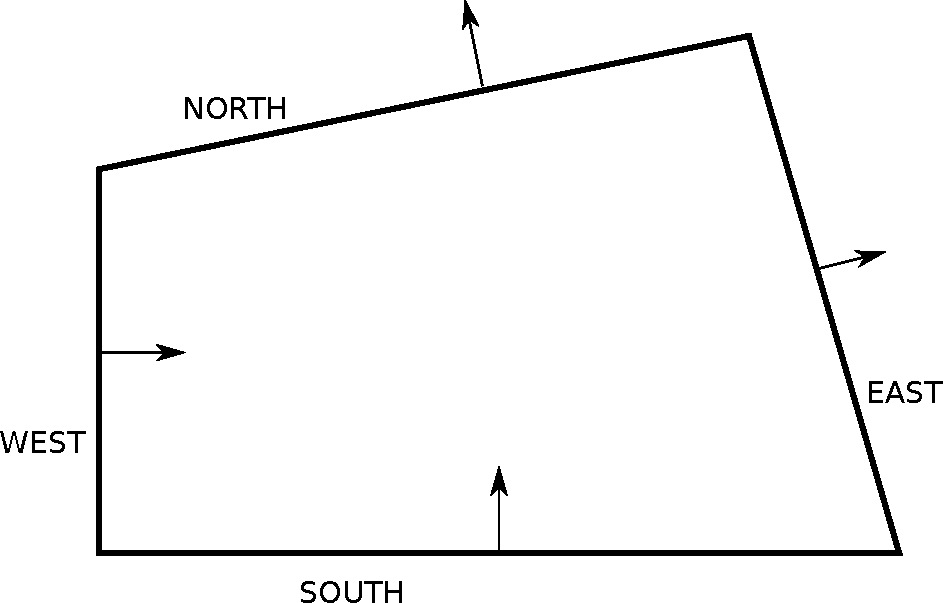
\includegraphics[width=10cm]{figs/boundary-normals.pdf}
\end{center}
\caption{The positive sense of direction for unit normals at each of the boundaries in 2D.}
\label{fig:boundary-normals}
\end{figure}

\medskip
The reason for this arrangement of face-normals is that, internal to the code, all \texttt{EAST}
and \texttt{WEST} interfaces are part of the single array of \texttt{i-faces}.
For \texttt{NORTH} and \texttt{SOUTH}, there is the single array of \texttt{j-faces} and,
for \texttt{TOP} and \texttt{BOTTOM} faces, there is the array of \texttt{k-faces}.
So, a single \texttt{i-face} will serve as the \texttt{EAST} face of one cell and 
the \texttt{WEST} face of the next cell to its right.


\subsection{Source terms}
\label{source-terms-udf}
\index{source terms!user defined}
%
The Python input script can also specify the filename for a Lua file that contains functions
that can be called to specify additional source terms for each step of the simulation.
The functions \textit{expected} to be defined are \texttt{source\_vector(t, cell)},
\texttt{at\_timestep\_start(args)} and \texttt{at\_timestep\_end(args)}.
If you don't have any useful work for the latter two, just define them to return \texttt{nil}.
These latter two functions are described in Section~\ref{start-end-timestep-udf}.
The Lua execution environment provided provided to the file includes the following data:\\
\begin{tabular}{ll}
 \texttt{nsp} & number of species \\
 \texttt{nmodes} & number of energy storage modes (and temperatures) \\
 \texttt{sample\_flow} & \parbox{12cm}{a function that returns a table of 
                                      the flow state for a particular cell} \\
 \texttt{locate\_cell} & \parbox{12cm}{a function that will search for the cell nearest 
                                      the specified coordinates and return the cell indices
                                      and the index of the containing block} 
\end{tabular}
 
\bigskip
When activated, the function \texttt{source\_vector(t, cell)} will be called at each time step.
The first argument, \texttt{t}, is the current simulation time, in seconds.
The table \texttt{cell} contains:\\
\begin{tabular}{ll}
 \texttt{x,y,x} & coordinates of the cell centre \\
 \texttt{vol} & cell volume \\
 \texttt{p} & gas pressure \\
 \texttt{rho} & gas density \\
 \texttt{u,v,w} & gas velocity components \\
 \texttt{a} & speed of sound in gas \\
 \texttt{mu} & gas viscosity \\
 \texttt{T} & table of \texttt{nmodes} temperatures \\
 \texttt{k} & table of \texttt{nmodes} thermal conductivities \\
 \texttt{massf} & table of \texttt{nsp} mass fractions \\
\end{tabular}\\
On return, the table of source terms should contain:\\
\begin{tabular}{ll}
 \texttt{mass} &  rate of mass addition per unit volume\\
 \texttt{momentum\_x} & rate of x-momentum addition per unit volume\\
 \texttt{momentum\_y} & rate of y-momentum addition per unit volume\\
 \texttt{momentum\_z} & rate of z-momentum addition per unit volume\\
 \texttt{total\_energy} & rate of energy addition per unit volume\\
 \texttt{romega} & $d\omega/dt$ addition per unit volume\\
 \texttt{rtke} & rate of turbulent kinetic-energy addition per unit volume\\
 \texttt{radiation} & rate of energy addition via radiation per unit volume\\
 \texttt{species} & table of \texttt{nsp} values\\
 \texttt{energies} & table of \texttt{nmodes} values\\
\end{tabular}\\

\subsection{Callable functions at timestep start and timestep end}
\label{start-end-timestep-udf}
The callable functions at timestep start and timestep end differ
from the user-defined boundary conditions and user-defined source terms
in two key ways:
\begin{enumerate}
\item the functions are only called once on each timestep iteration; and
\item the functions are used to extract information from the flow field
      but cannot alter its state in anyway (nothing is returned to the
      C++ code)
\end{enumerate}

In the case of the callable boundary conditions, the functions are called many times
each timestep for each of the interfaces.
Similarly, the callable source vector function is called once for every cell in 
the flow field.
However, the user-defined functions \verb!at_timestep_start()! and \verb!at_timestep_end()!
are only called once in each iteration.
As such, if the user would like to gather data from all cells,
then the user is responsible for looping over those cells.

In the present implementation, we do not provide a mechanism to alter the
state of the cells and boundaries in the flow field via the functions
\verb!at_timestep_start()! and \verb!at_timestep_end()!.
The callable functions are only intended to extract information from the
flowfield.\footnote{Note the cunning user could use all of the Lua callable functions
to affect the flow field.
For example, the user could extract certain information from
the flow field using the \texttt{at\_timestep\_end()} hook, make a decision based on that information,
write some data to a local file and then have a user-defined boundary condition pick
up and act on that data.
An early implementation of a conjugate heat transfer boundary
condition was done in a similar manner to this.}

The global Lua environment for the \verb!at_timestep_start()! and \verb!at_timestep_end()!
functions is the same as that for the user-defined source terms (see Section~\ref{source-terms-udf}).
When either function is called, it is passed a table of arguments from the flow solver.
That table contains:\\
\begin{tabular}{ll}
 \texttt{t} & current simulation time in seconds \\
 \texttt{step} & current step number in simulation \\
 \texttt{nblks} & number of blocks in simulation \\
 \texttt{nrank} & rank number, only meaningful in MPI simulations \\
 \texttt{blks} & a table containing information for each block, explained below \\
\end{tabular}\\
One of the arguments, \verb!blks!, is itself a table (in particular, an array) containing information 
about each of the blocks individually.
To access the information in the second block, for example, you could interrogate
the table \verb!blks[1]!, using 1 for the second block because of 0-offset indexing.
So each entry in \verb!blks! is a table itself --- that's right tables within tables within
tables. Each table within \verb!blks! contains the following information about a particular
block:\\
\begin{tabular}{ll}
 \texttt{nicells} & number of cells in $i$-direction \\
 \texttt{imin} & index of minimum cell number in $i$-direction \\
 \texttt{imax} & index of maximum cell number in $i$-direction \\
 \texttt{njcells} & number of cells in $j$-direction \\
 \texttt{jmin} & index of minimum cell number in $j$-direction \\
 \texttt{jmax} & index of maximum cell number in $j$-direction \\
 \texttt{nkcells} & number of cells in $k$-direction \\
 \texttt{kmin} & index of minimum cell number in $k$-direction \\
 \texttt{kmax} & index of maximum cell number in $k$-direction \\
\end{tabular}

The brief example below shows how we could loop over all the cells in a flowfield
and get a tally of the total mass at the start
of the first timestep using the \verb!at_timestep_Start()! function.

\begin{verbatim}
function at_timestep_start(args)
    if (args.step ~= 0) then
        -- do nothing, just leave
        return
    end
    -- For the 0th step only
    nblks = args.nblks
    blks = args.blks
    mass = 0.0
    for ib=0,(nblks-1) do
        imin = blks[ib].imin; imax = blks[ib].imax
        jmin = blks[ib].jmin; jmax = blks[ib].jmax
        kmin = blks[ib].kmin; kmax = blks[ib].kmax
        for k=kmin,kmax do
            for j=jmin,jmax do
                for i=imin,imax do
                    cell = sample_flow(ib, i, j, k)
                    -- We are only given p and T
                    -- so need to compute density
                    -- using gas model
                    Q = create_empty_gas_table()
                    Q.p = cell.p
                    Q.T = cell.T
                    for isp=0,(nsp-1) do Q.massf[isp] = cell.massf[isp] end
                    eval_thermo_state_pT(Q)
                    rho = Q.rho
                    -- Now we can compute mass in cell using volume of cell
                    mass = mass + rho*cell.vol
                end
            end
        end
    print("Mass (kg) of gas in domain: ", mass)
    return
end
\end{verbatim}

There's a little bit to digest in the example above. 
We'll begin with the \verb!if!-statement.
Remember that the \verb!at_timestep_start()! is called for
every timestep, which means we enter this piece of code
on every iteration.
However we only want to compute the mass at
the very beginning of the simulation.
So, the \verb!if!-statement says that if we are \emph{not}
at step 0 (the beginning step), then do nothing and move on.
The code only continues then in the case where the
step number is equal to 0.

In the case where the step number is 0, we want to loop
over all cells and tally the mass.
To do that, we firstly need to know how many blocks there are in the
simulation. (Admittedly, we might know how many blocks there
are already because we set the simulation up ourselves!
However, by keeping the code general we can reuse it
for other simulations without alterting the Lua code.)
We can get the number of blocks from the supplied entry
\verb!nblks! in the table of arguments.
Then we loop over all blocks using the \verb!ib! variables
as a counter for the block index.
Within any particular block, we want to loop over the
simulation cells only, and exclude any ghost cells at
the boundaries.
The appropriate ranges for the simulation cells
in each of the $i$-, $j$- and $k$-directions are
given by the \verb!min! and \verb!max! variables
within each block table.
Having extracted those values, we can set up
loops to visit every simulation cell in a block.

In the inner most loop, we visit every cell
and extract its density and volume so that we
can compute the mass in the cell.
We call the \verb!sample_flow()! function to get
the information of a single cell.
To compute the density is a little complicated.
We are only given pressure, temperature and 
species mass fractions.
The provided gas model functions are used
to compute density.
For the moment, don't worry too much about the
details of making the calculation to get density.
These functions are explained later in Section~\ref{sec:udf-gas-service}.
The volume is easy to get: we extract directly from the
cell as variable \verb!vol!.
In the last step, we compute the mass in this cell ($\rho \times V$)
and add it to the total.


\subsection{Helper gas model functions}
\label{sec:udf-gas-service}

There are a large number of functions provided by the gas module to the internal
(C++) section of the code.
For consistency with the internal gas model, a selection of the gas module
functions are made available to the Lua run-time scripts.
The names of these Lua-exposed functions match the internal C++ names very
closely (and in fact, identically in most cases).
The provided gas model functions are:\\
\begin{tabular}{p{6.2cm}p{10cm}} 
 \noalign{\smallskip} \hline \noalign{\smallskip}
 \texttt{create\_empty\_gas\_table()} & Returns an empty \texttt{Gas\_data} table with all entries set to 0.0 and appropriately sized internal arrays. This is useful to populate and pass to other functions which accept a \texttt{Gas\_data} table. \\
 \texttt{eval\_thermo\_state\_pT(Q)} & A function that computes the thermodynamic state given the pressure and temperatures as set in the \texttt{Gas\_data} table \texttt{Q}. The thermodynamic properties are updated and returned in place in the \texttt{Q} variable, that is, it is modified in place. \\
 \texttt{eval\_thermo\_state\_rhoe(Q)} & A function that computes the thermodynamic state given density and internal energy. The \texttt{Gas\_data} table \texttt{Q} is modified in place. \\
 \texttt{eval\_thermo\_state\_rhoT(Q)} & A function that computes the thermodynamic state given density and temperatures. The \texttt{Gas\_data} table \texttt{Q} is modified in place. \\
\texttt{eval\_thermo\_state\_rhop(Q)} & A function that computes the thermodynamic state given density and pressure. The \texttt{Gas\_data} table \texttt{Q} is modified in place. \\
\texttt{eval\_sound\_speed(Q)} &  A function that computes the sound speed based on the supplied thermodynamic state in \texttt{Q}. The \texttt{Gas\_data} table \texttt{Q} is modified in place such \texttt{Q.a} contains the computed
sound speed value. \\
\texttt{eval\_transport\_coefficients(Q)} & A function that computes the
transport coefficients, viscosity and thermal conductivities, based on the
supplied gas state in \texttt{Q}. The \texttt{Gas\_data} table \texttt{Q} is
modified in place so that \texttt{Q.mu} and \texttt{Q.k[]} are up to date. \\
\texttt{eval\_diffusion\_coefficients(Q)} & A function that computes the
diffusion coefficients for interacting species pairs based on the
thermodynamic state in \texttt{Q}. The values in \texttt{Q.D[][]} are modified
in place so that they are up to date. \\
\texttt{eval\_Cv(Q)} & A function that returns (as a double)
the mixture specific heat at constant volume (in J/(kg.K)) based
on the supplied thermodynamic state in \texttt{Q}. \\
\texttt{eval\_Cp(Q)} & A function that returns (as a double)
the mixture specific heat at constant pressure (in J/(kg.K)) based
on the supplied thermodynamic state in \texttt{Q}. \\
\texttt{eval\_R(Q)} & A function that returns (as a double)
the mixture gas constant (in J/(kg.K)) based
on the supplied thermodynamic state in \texttt{Q}. \\
\texttt{eval\_gamma(Q)} & A function that returns (as a double)
the ratio of specific heats (non-dimensional) based
on the supplied thermodynamic state in \texttt{Q}. \\
\noalign{\smallskip} \hline \noalign{\smallskip}
\end{tabular}
\\
\begin{tabular}{p{5cm}p{9cm}} 
 \noalign{\smallskip} \hline \noalign{\smallskip}
\texttt{molecular\_weight(isp)} & A function that returns
the molecular weight of species number \texttt{isp}. The
units of molecular weight is returned in kg/mol because this
is consistent with the internal units of the code. Note that
the units of molecular weight listed on the Periodic Table
and commonly used in textbook formulas is in g/mol. The returned
value should be multiplied by 1000.0 to give g/mol. \\
\texttt{massf2molef(massf)} & A function that returns a table
of mole fractions based on a supplied table of mass fractions.
Note the table of supplied mass fractions must be the full size
of the number of species in the gas model. Similarly, the returned
mole fractions table has values for all participating species. \\
\texttt{molef2massf(molef)} & A function that returns a table
of mass fractions based on a supplied table of mole fractions.
Note the table of supplied mole fractions must be the full size
of the number of species in the gas model. Similarly, the returned
mass fractions table has values for all participating species. \\
\texttt{massf2conc(rho, massf)} & A function that returns a table
of concentrations (mol/m$^3$) based on a supplied density and
table of mass fractions.
Note the table of supplied mass fractions must be the full size
of the number of species in the gas model. Similarly, the returned
concentrations table has values for all participating species. \\
\texttt{conc2massf(rho, conc)} & A function that returns a table
of mass fractions based on a supplied density and table of concentrations
in mol/m$^3$.
Note the table of supplied concentrations must be the full size
of the number of species in the gas model. Similarly, the returned
mass fraction table has values for all participating species. \\
\noalign{\smallskip} \hline \noalign{\smallskip}
\end{tabular}

\subsection{Notes on global variables and Lua interpreters}
%
For each boundary condition that uses a \verb!USER-DEFINED! boundary condition, 
an independent Lua interpreter is started. 
The global state in each of these interpreters (read boundary conditions) 
is kept between timesteps (\textit{i.e.} the interpreter is reentrant). 
However, there is no way to communicate information internally from one Lua interpreter to another. 
There is a subtlety here. 
You could actually write just one Lua file as the boundary condition but set it on multiple boundaries 
however, you would need to make it smart enough to use the Eilmer-provided information to work out 
which boundary it was and then act accordingly. 
Remember that, although you might use the one file, 
it is running as an independent process for each boundary. 
Those independent processes will not share global state and cannot communicate.

\medskip
An independent Lua interpreter is also started when using the global \verb!udf_file! 
to supply \verb!at_timestep_start()! and \verb!at_timestep_end()! functions. 
A single interpreter is started to house both those functions and 
the global state in that interpreter is also reentrant. 


